%!TEX root = Economics and Behaviour.tex

\section{Sub-game-Perfect Nash-Equilibrium}

The Dictator-Game is nicely analysed by Christoph Engel in his book \textit{Dictator-Games: A meta study (2011)}. In the following part we'd like to look at a modification of the Dictator-Game:

\begin{example}[Ultimatum-Game]	\label{ultimatumgame} \index{Ultimatum-Game} 
The Ultimatum-Game is a dynamic game under complete information. \\
We look at two players in two stages. The first player (the proposer (P)) receives a sum of money $(M = 10)$ and proposes how to divide the sum between himself $(x_{p})$, where $x_{p} \in \{ 0, 1, 2, \dotsc, 10 \}$, and another player $(10 - x_{p})$. The second player (the responder (R)) chooses to either accept or reject this proposal. If the second player accepts, the money is split according to the proposal. If the second player reject, neither player receives any money.

Lets sum this up again:
	\begin{itemize}
		\item P proposes split up $(x_{p}, 10 - x_{p})$
		\item R accepts or rejects
			\begin{itemize}
				\item If R accepts $(a)$, proposal becomes implemented. P receives $x_{p}$ and R $10 - x_{p}$
				\item If R rejects $(r)$, the whole money gets destroyed.
			\end{itemize}
	\end{itemize}
	
	\begin{center}
		\begin{tikzpicture}[auto,level 1/.style={sibling distance=35mm/#1}, level distance=30mm]
			\node [circle,draw] (z){$P$}
 						child {node [circle,draw] (a) {$10$}	}
 						child {node [] (b) {$ $}	}
 						child {node [circle,draw] (c) {$x_{p}$}
  							child {node [circle,draw] (f) {$(x_{p}, 10 - x_{p})$}	}
  			 				child {node [circle,draw] (g) {$(0, 0)$}	}			
 						}
 						child {node [] (d) {$$}	}
  						child {node [circle,draw] (e) {$0$}
			};
			\path (a) -- (b) node [midway] {$\dotsc$};
			\path (b) -- (c) node [midway] {$\dotsc$};
			\path (c) -- (d) node [midway] {$\dotsc$};
			\path (d) -- (e) node [midway] {$\dotsc$};
			\path (f) -- (g) node [midway] {$a$ $/$ $r$};
		\end{tikzpicture}				
	\end{center}
	
	A strategy set in this game would have to look like
	\begin{itemize}
		\item Proposer sets a $x_{p}$
		\item Receiver decides for \textit{any} $x_{p}$ that might come up if he'd accept or reject that offer.
	\end{itemize}
	\begin{center}( a strategy needs to specify a complete action plan. ) \end{center}
	
	
	\textbf{1. Question:} Can the outcome $(5, 5)$ be stabilised as a Nash-Equilibrium outcome? \\
	\textbf{Answer:} Yes. Say P proposes $x_{p} = 5$ and the strategy set for R is defined by accepting for any value of $x_{p} \leq 5$ and rejecting the offer for values larger then $5$. \\
		In this situation $(5, 5)$ would be stabilised as a Nash-Equilibrium.


	\textbf{2. Question:} Is there another Nash-Equilibrium that stabilises the $(5, 5)$ outcome? \\
	\textbf{Answer:} Yes. If P again proposes $x_{p} = 5$ and the strategy set for R is defined by accepting for only $x_{p} = 5$ and rejecting for any other case, so $x_{p} \neq 5$. 
	
	
	\textbf{3. Question:} Can $(0, 10)$ be stabilised as a Nash-Equilibrium? \\
	\textbf{Answer:} Yes. We set the strategy for P as $x_{p} = 0$ and for R demand accepting for $x_{p} = 0$ and rejecting for any other case, meaning for $x_{p} \geq 1$. 
\end{example}

As we can see the Nash-Equilibrium can lead to an infinite amount of outcomes some of them even with implausible threats. We'd therefore would like to refine this kind of equilibrium which leads to the (sub-game) perfect Nash-Equilibrium.

\begin{definition}[Sub-game] \index{sub-game}
	A sub-game is any part of a game that meets the following criteria:
	\begin{itemize}
		\item It has a single initial node that is the only member of that node's information set (i.e. the initial node is in a singleton information set).
		\item If a node is contained in the sub-game then so are all of its successors
		\item If a node in a particular information set is in the sub-game then all members of that information set belong to the sub-game.
	\end{itemize}
\end{definition}

\begin{definition}[(Sub-game-)Perfect Nash-Equilibrium] \index{Sub-game-Perfect Nash-Equilibrium} 
A strategy profile is a Sub-game-Perfect Nash-Equilibrium if it represents a Nash equilibrium of every sub-game of the original game. Informally, this means that if the players played any smaller game that consisted of only one part of the larger game and their behaviour represents a Nash equilibrium of that smaller game, then their behaviour is a sub-game perfect equilibrium of the larger game. 

	How to find a Perfect Nash-Equilibrium:
	\begin{enumerate}
		\item Define (one set of) optimal actions for the last sub-game
		\item Replace that decision nodes with the respective outcome
		\item Repeat $(1)$ and $(2)$ until the first decision node.
	\end{enumerate}
\end{definition}

\begin{example}[Sequel to the Ultimatum-Game]
	Searching for the Perfect Nash-Equilibrium in this case leads to:
	\begin{enumerate}
		\item Defining the optimal actions
			\begin{itemize}
				\item In the case $P$ chooses $x_{p} = 10$, then $R$ receives  $10 - x_{p} = 0$ and he is 	indifferent between refusing and accepting. Let's assume for now he'd accept in this case.
				\item In all other cases, meaning $x_{p} \in [0, 10)$, would R receive $10 - x_{p} > 0$. Therefore he would accept the offer in all cases.
			\end{itemize}
		\item Now we can reduce the game to the following game tree
			\begin{center}
				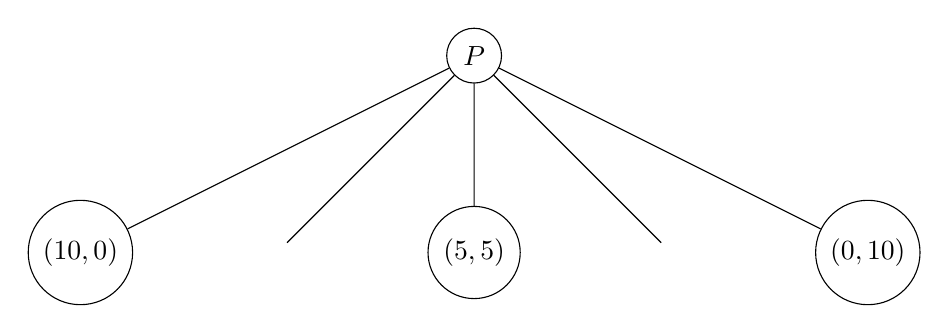
\begin{tikzpicture}[level/.style={sibling distance=25mm/#1}, level 	distance=25mm]
					\node [circle,draw] (z){$P$}
 						child {node [circle,draw] (a) {$(10, 0)$}	}
 						child {node [] (b) {$ $}	}
 						child {node [circle,draw] (c) {$(5, 5)$}	}
 						child {node [] (d) {$ $}	}
  						child {node [circle,draw] (e) {$(0, 10)$}
					};
					\path (a) -- (b) node [midway] {$\dotsc$};
					\path (b) -- (c) node [midway] {$\dotsc$};
					\path (c) -- (d) node [midway] {$\dotsc$};
					\path (d) -- (e) node [midway] {$\dotsc$};
				\end{tikzpicture}				
			\end{center}
		\item In the reduced game we have already reached the first node and can now analyse the situation for Nash-Equilibriums. Here $P$ choses $x_{p} = 10$ since it results in his highes utility.
	\end{enumerate}
	$\Rightarrow P$ plays $x_{p} = 10$ together with R always accepts constitutes a Sub-game-Perfect Nash-Equilibrium. 

	If we'd look for another equilibrium it yields
		\begin{enumerate}
		\item the optimal actions
			\begin{itemize}
				\item Again, in all cases $x_{p} \in [0, 10)$ would R receive $10 - x_{p} > 0$, therefore he'd accept the offer in all cases.
				\item If he now would refuse to the offer $x_{p} = 10$ it would be plausible therefore sub-game perfect, since he indifferent between both choices.
			\end{itemize}
		\item the tree changes only slightly:
			\begin{center}
				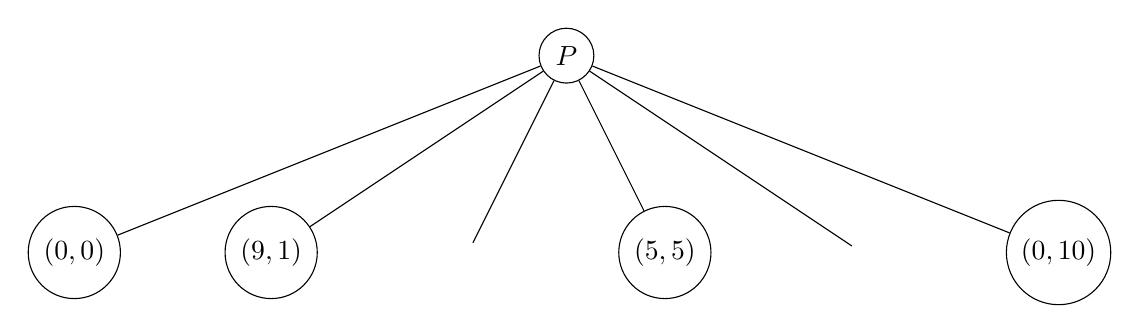
\begin{tikzpicture}[level/.style={sibling distance=25mm/#1}, level 	distance=25mm]
					\node [circle,draw] (z){$P$}
 						child {node [circle,draw] (a) {$(0, 0)$}	}
 						child {node [circle,draw] (b) {$(9, 1)$}	}
 						child {node [] (c) {$ $}	}
 						child {node [circle,draw] (d) {$(5, 5)$}	}
 						child {node [] (e) {$ $}	}
  						child {node [circle,draw] (f) {$(0, 10)$}
					};
					\path (b) -- (c) node [midway] {$\dotsc$};
					\path (c) -- (d) node [midway] {$\dotsc$};
					\path (d) -- (e) node [midway] {$\dotsc$};
					\path (e) -- (f) node [midway] {$\dotsc$};
				\end{tikzpicture}				
			\end{center}
	\end{enumerate}
	$\Rightarrow P$ plays $x_{p} = 9$ together with R always accepts if $x_{p} < 10$ and refuses for $x_{p} = 10$ constitutes also a Sub-game-Perfect Nash-Equilibrium. 
\end{example}

\subsection{Presentations}
todo %todo: have to sum those presentations up

\newpage